\documentclass[11pt]{article}
\usepackage{geometry}
\usepackage{graphicx}
\usepackage{wrapfig}
\usepackage{float}
\usepackage{caption}
\usepackage{subcaption}
\usepackage[T1]{fontenc}
\usepackage[utf8]{inputenc}
\usepackage{helvet}
\renewcommand{\familydefault}{\sfdefault}
%\usepackage{titlesec}
%\titlespacing\section{1pt}{12pt plus 2pt minus 2pt}{1pt plus 2pt minus 2pt}
%\titlespacing\subsection{1pt}{12pt plus 2pt minus 2pt}{pt plus 2pt minus 2pt}
%\titlespacing\subsubsection{5pt}{12pt plus 2pt minus 2pt}{1pt plus 2pt minus 2pt}
%\usepackage{float}
\usepackage[hidelinks]{hyperref}
\usepackage{hyperref}
\usepackage{float}
\hypersetup{
	colorlinks=true,
	linkcolor=blue,
	filecolor=magenta,      
	urlcolor=cyan,
	pdftitle={Overleaf Example},
	pdfpagemode=FullScreen,
}

\urlstyle{same}
\geometry{margin=0.5in}
%opening
%\titleformat*{\section}{\small\bfseries}
\bibliographystyle{unsrt}
\author{Ethan Holleman}
\title{Variable region design and cloning protocol outline}
\usepackage{booktabs}
\begin{document}

\maketitle


\section{Insert design overview}

The overall goal of this series of experiments is to transcribe carefully controlled DNA sequences, referred to as inserts, in order to systematically observe the effects of these sequences on R-loop formation \emph{in vitro}. Inserts are composed of two types of DNA components, the variable region and flanking infrastructure regions. The variable region contains the sequence we are interested in observing R-loop dynamics over. Infrastructure sequences are additional nucleotide blocks that allow for the insertion of variable regions into specific plasmid backbones in a modular fashion. 

\begin{figure}[h]
	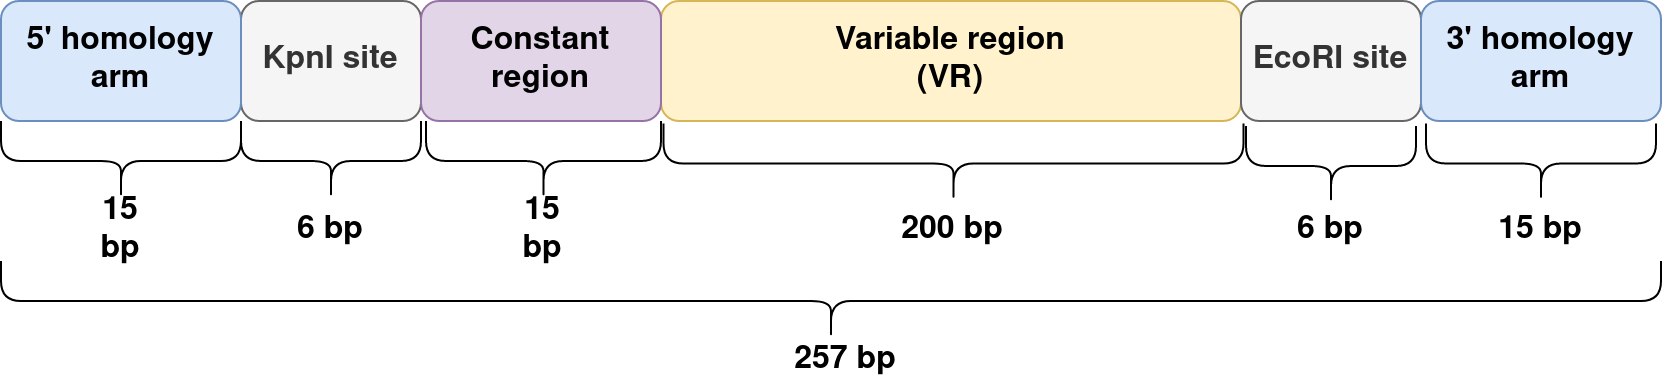
\includegraphics[width=16cm]{images/variable_region_diagram.png}
	\centering
	\caption{Diagram of a complement variable region insert showing the various regions each complete insert will contain, their relative order and lengths.}
	\label{fig:1}
\end{figure}

Each insert will be completely synthesized by an outside manufacturer and will not require assembly. 

\subsection{Variable regions}

As is shown fig. \ref{fig:1} each insert will contain 1 variable region which will be designed to test the effects of different sequence properties on R-loop dynamics, namely GC / AT skew, GC content and G / C clustering. In total, 29 different variable regions with the properties described in table \ref{table:1} will be generated using the \href{https://github.com/EthanHolleman/plasmid-VR-design}{variable region design workflow}. The same pipeline will then be used to prepend or append infrastructure sequences to each variable region in order to produce a final fasta file containing the complete sequence of all inserts that can then be ordered for synthesis. The inserts will first be used to study the impact of sequence variation on R-loop initiation by insertion directly downstream of a promoter.

\begin{table}
\centering
\caption{Properties of all syntheized inserts. The G clustering number refers to the number of G nucleotides in a given cluster with 0 being no clustering.}
\label{table:1}
\begin{tabular}{rrrrrr}
\toprule=
 GC Skew &  AT Skew &  GC Content &  G Clustering &  Reverse Complement &  Insert Number \\
\midrule
     0.2 &      0.0 &         0.4 &             0 &                   1 &              0 \\
     0.1 &      0.0 &         0.3 &             0 &                   0 &              1 \\
     0.6 &      0.0 &         0.6 &             0 &                   0 &              2 \\
     0.4 &      0.0 &         0.3 &             0 &                   1 &              3 \\
     0.2 &      0.0 &         0.3 &             0 &                   1 &              4 \\
     0.0 &      0.0 &         0.3 &             0 &                   1 &              5 \\
     0.0 &      0.0 &         0.6 &             0 &                   0 &              6 \\
     0.6 &      0.0 &         0.5 &             0 &                   0 &              7 \\
     0.1 &      0.0 &         0.6 &             0 &                   0 &              8 \\
     0.4 &      0.0 &         0.6 &             0 &                   0 &              9 \\
     0.2 &      0.0 &         0.6 &             0 &                   0 &             10 \\
     0.0 &      0.0 &         0.5 &             0 &                   1 &             11 \\
     0.6 &      0.0 &         0.4 &             0 &                   0 &             12 \\
     0.0 &      0.0 &         0.4 &             0 &                   1 &             13 \\
     0.1 &      0.0 &         0.5 &             0 &                   0 &             14 \\
     0.6 &      0.0 &         0.3 &             0 &                   0 &             15 \\
     0.4 &      0.0 &         0.5 &             0 &                   1 &             16 \\
     0.2 &      0.0 &         0.5 &             0 &                   1 &             17 \\
     0.1 &      0.0 &         0.4 &             0 &                   0 &             18 \\
     0.4 &      0.0 &         0.4 &             0 &                   1 &             19 \\
     0.4 &      0.0 &         0.6 &             2 &                   1 &             20 \\
     0.4 &      0.2 &         0.6 &             2 &                   1 &             21 \\
     0.4 &      0.4 &         0.6 &             2 &                   1 &             22 \\
     0.4 &      0.0 &         0.6 &             3 &                   1 &             23 \\
     0.4 &      0.2 &         0.6 &             3 &                   1 &             24 \\
     0.4 &      0.4 &         0.6 &             3 &                   1 &             25 \\
     0.4 &      0.0 &         0.6 &             4 &                   1 &             26 \\
     0.4 &      0.2 &         0.6 &             4 &                   1 &             27 \\
     0.4 &      0.4 &         0.6 &             4 &                   1 &             28 \\
\bottomrule
\end{tabular}
\end{table}


A subset of the variable regions will also be cloned further downstream of the same promoter species and oriented so the reverse complement of the sequence is transcribed in order to access their capacity for R-loop termination. The properties of the transcripts of these sequences are listed in table \ref{table:2}. 

\begin{table}[H]
\centering
\caption{}
\label{table:2}
\begin{tabular}{rrrrr}
\toprule
 GC Skew &  AT Skew &  GC Content &  C Clustering &  Reverse Complement of Insert \\
\midrule
    -0.2 &     -0.0 &         0.4 &             0 &                             0 \\
    -0.4 &     -0.0 &         0.3 &             0 &                             3 \\
    -0.2 &     -0.0 &         0.3 &             0 &                             4 \\
    -0.0 &     -0.0 &         0.3 &             0 &                             5 \\
    -0.0 &     -0.0 &         0.5 &             0 &                            11 \\
    -0.0 &     -0.0 &         0.4 &             0 &                            13 \\
    -0.4 &     -0.0 &         0.5 &             0 &                            16 \\
    -0.2 &     -0.0 &         0.5 &             0 &                            17 \\
    -0.4 &     -0.0 &         0.4 &             0 &                            19 \\
    -0.4 &     -0.0 &         0.6 &             2 &                            20 \\
    -0.4 &     -0.2 &         0.6 &             2 &                            21 \\
    -0.4 &     -0.4 &         0.6 &             2 &                            22 \\
    -0.4 &     -0.0 &         0.6 &             3 &                            23 \\
    -0.4 &     -0.2 &         0.6 &             3 &                            24 \\
    -0.4 &     -0.4 &         0.6 &             3 &                            25 \\
    -0.4 &     -0.0 &         0.6 &             4 &                            26 \\
    -0.4 &     -0.2 &         0.6 &             4 &                            27 \\
    -0.4 &     -0.4 &         0.6 &             4 &                            28 \\
\bottomrule
\end{tabular}
\end{table}


The cloning experiments required to produce these termination constructs will be undertaken after initiation experiments are completed. This will allow for the identification of a strong initiation sequence, and the determination of the average length of R-loops formed within plasmid constructs. This will determine the placement of termination regions relative to the promoter as it is critical that termination regions are far enough downstream as to not interfere with R-loop initiation but also not so distant as to prevent R-loops from actually terminating within the termination region.

\begin{table}
\centering
\caption{}
\label{table:3}
\begin{tabular}{rr}
\toprule
 Total synthesized inserts &  Total contructs \\
\midrule
                        29 &               47 \\
\bottomrule
\end{tabular}
\end{table}




\section{Assembly of DNA inserts}

\subsection{Basic Strategy}

\begin{figure}[H]
	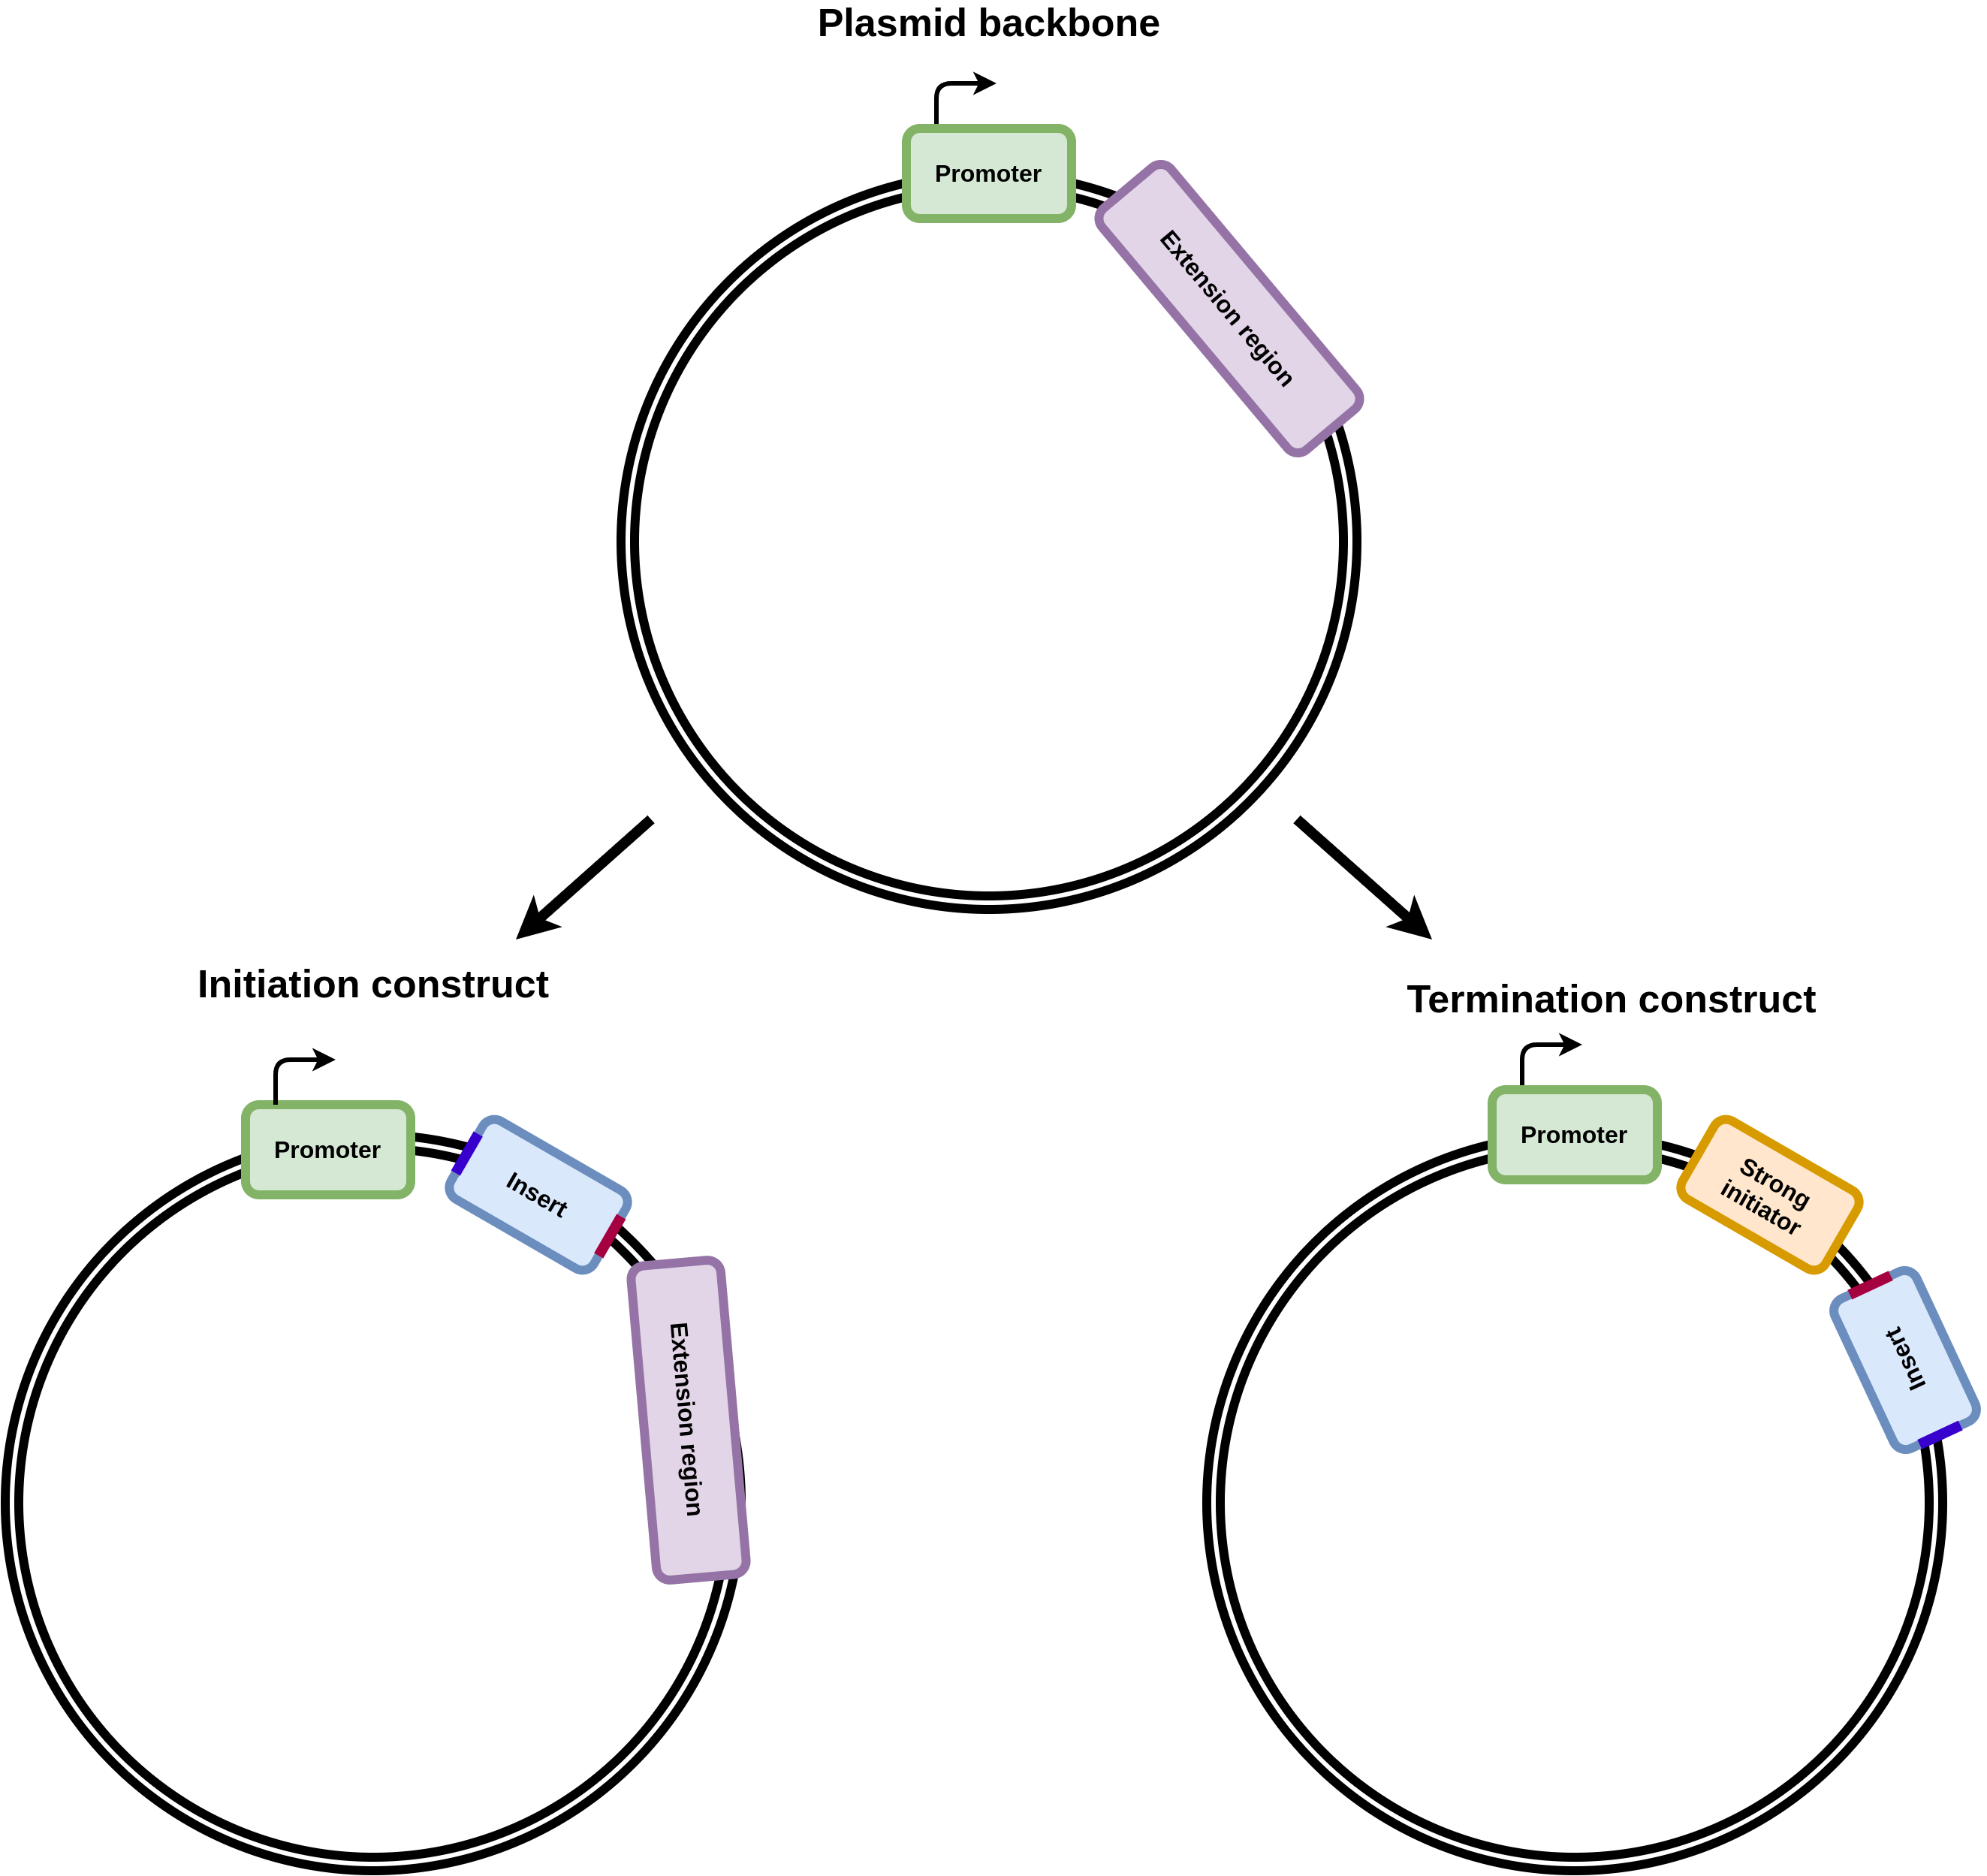
\includegraphics[width=10cm]{images/construct_diagram.png}
	\centering
	\caption{Diagram of basic cloning strategy. Inserts containing a variable region will be cloned into a backbone plasmid using either Gibson or restriction enzyme assembly to produce initiation or termination series constructs.}
\end{figure}

\subsection{T7 initiation series constructs}
\label{T7:init} 

The first series of constructs will be utilize pFC9 as the plasmid backbone.   

\begin{figure}[H]
	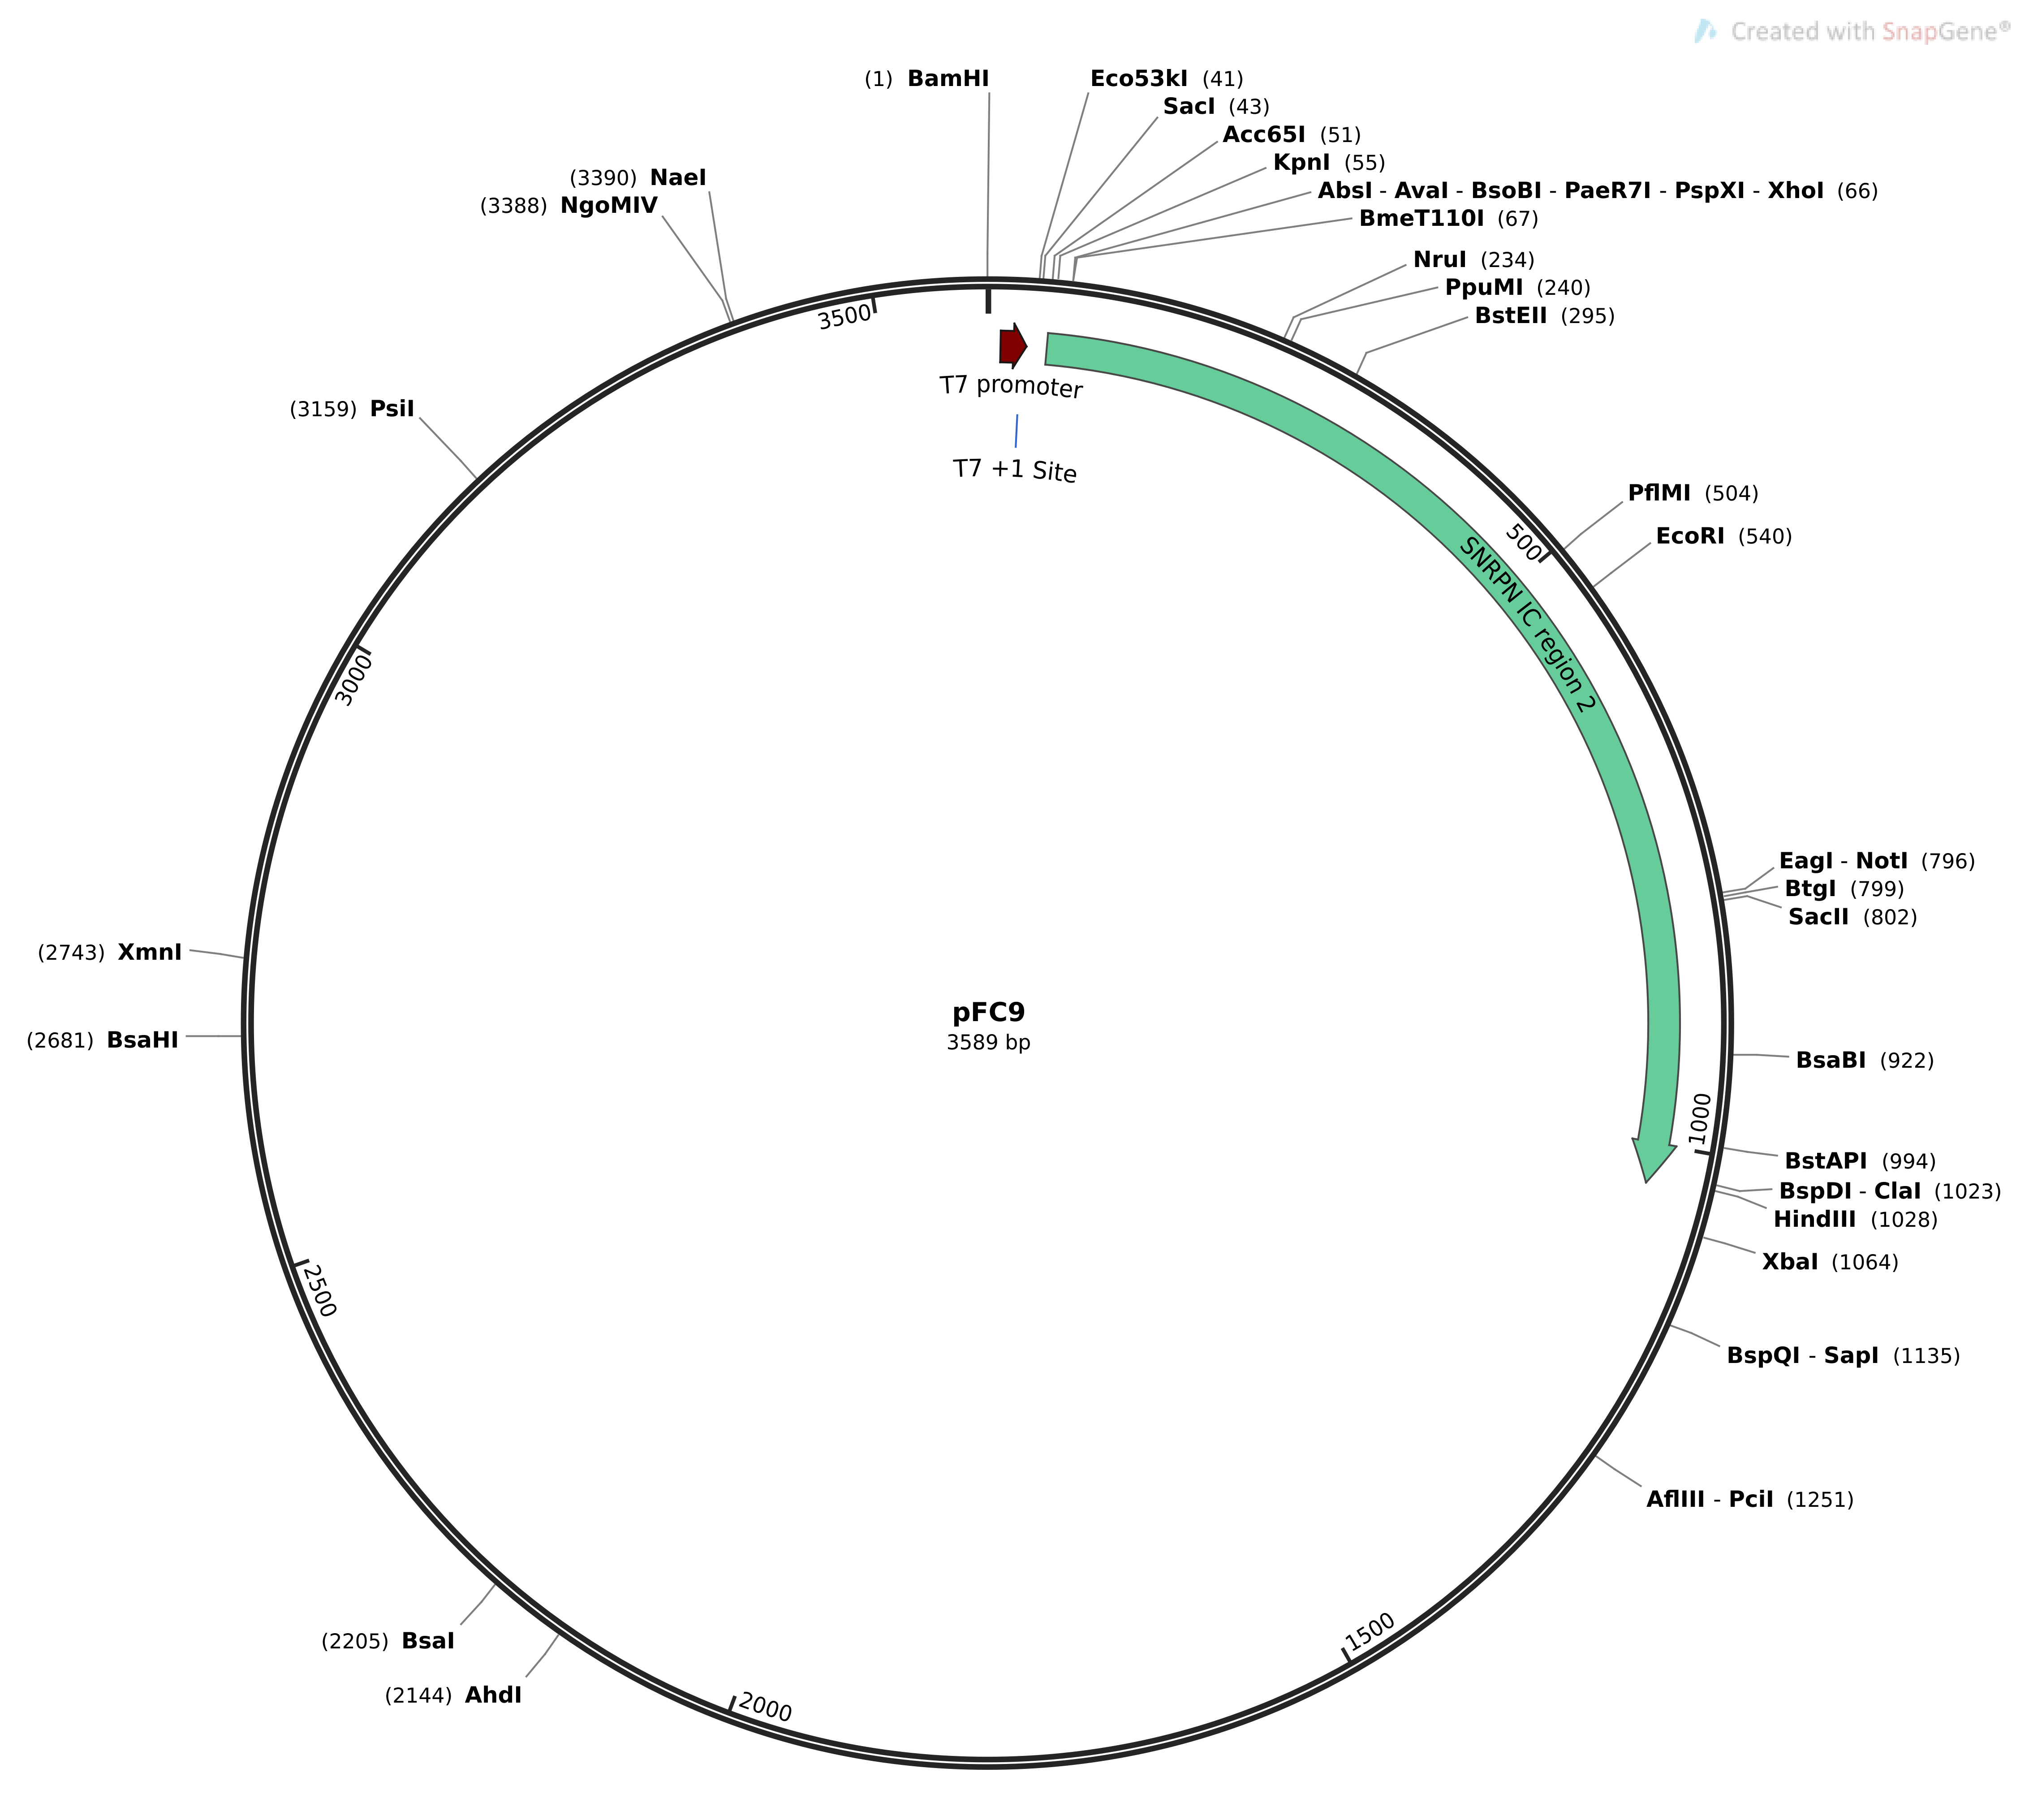
\includegraphics[width=10cm]{images/pFC9_Map.png}
	\centering
	\caption{Map of pFC9.}
	\label{fig:pFC9}
\end{figure}

First, pFC9 will be cut using Eco53KI, producing blunt ends just downstream of the T7 promotor (fig \ref{fig:pFC9}). The complete ensemble of inserts will then be added in equal concentrations. Using the \href{https://www.neb.com/protocols/2012/12/11/gibson-assembly-protocol-e5510}{NEB Gibson assembly kit and protocol}, the 5' and 3' homology arms will anneal to the T7 and extension region downstream of the Eco53KI cut site of pFC9 respectively producing a library of circular pFC9 plasmids with each insertion sequence in theoretically equivalent concentrations. 

\begin{figure}[h!]
	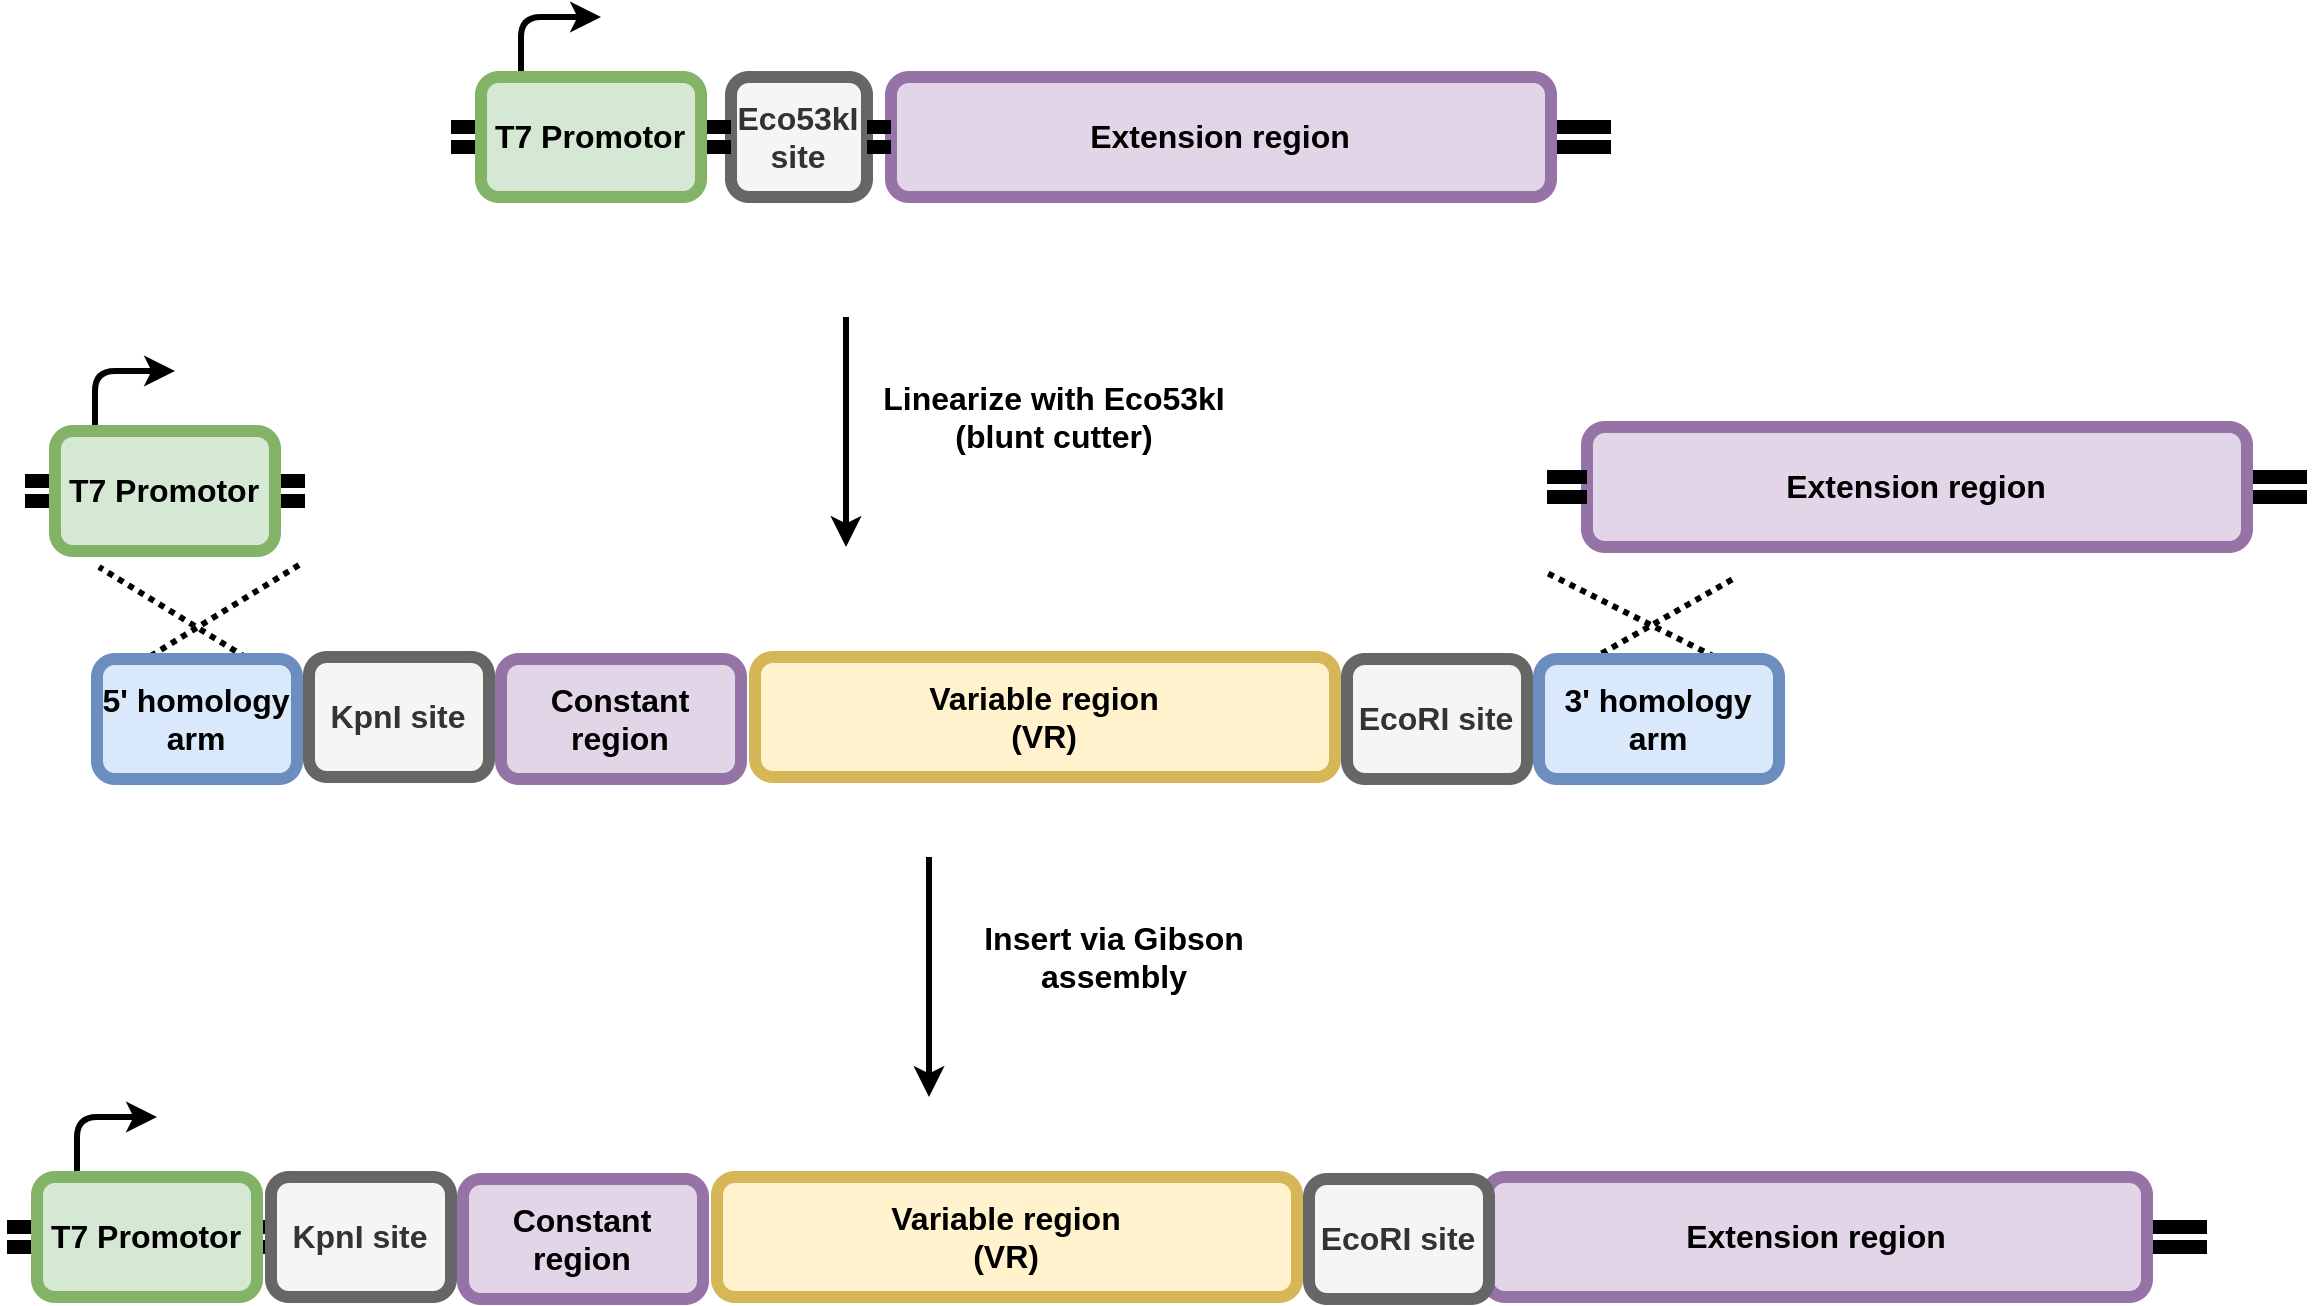
\includegraphics[width=15cm]{images/initiation_assembly_pFC9.png}
	\centering
	\caption{Diagram of pFC9 insertion series cloning strategy.}
\end{figure}

Additionally, primers will be designed for a subset of initiation regions and relative concentrations of each insert will be measured by qPCR. Having confirmed that inserts are present at relatively equal concentrations the library will be transcribed \emph{in vitro} and prepared for single molecule R-loop footprinting using uniquely bar-coded PCR primers to facilitate the computational removal of PCR duplicates. 


\subsection{T7 termination series constructs}

After the successful sequencing of the T7 initiation series, pFC8 will be utilized as the backbone for construction of the termination series library. First, the strongest and most consistent R-loop initiator identified from the T7 initiation series will be cloned into pFC9 without the presence of any other inserts using the methods described in section \ref{T7:init}. 

\begin{figure}[H]
	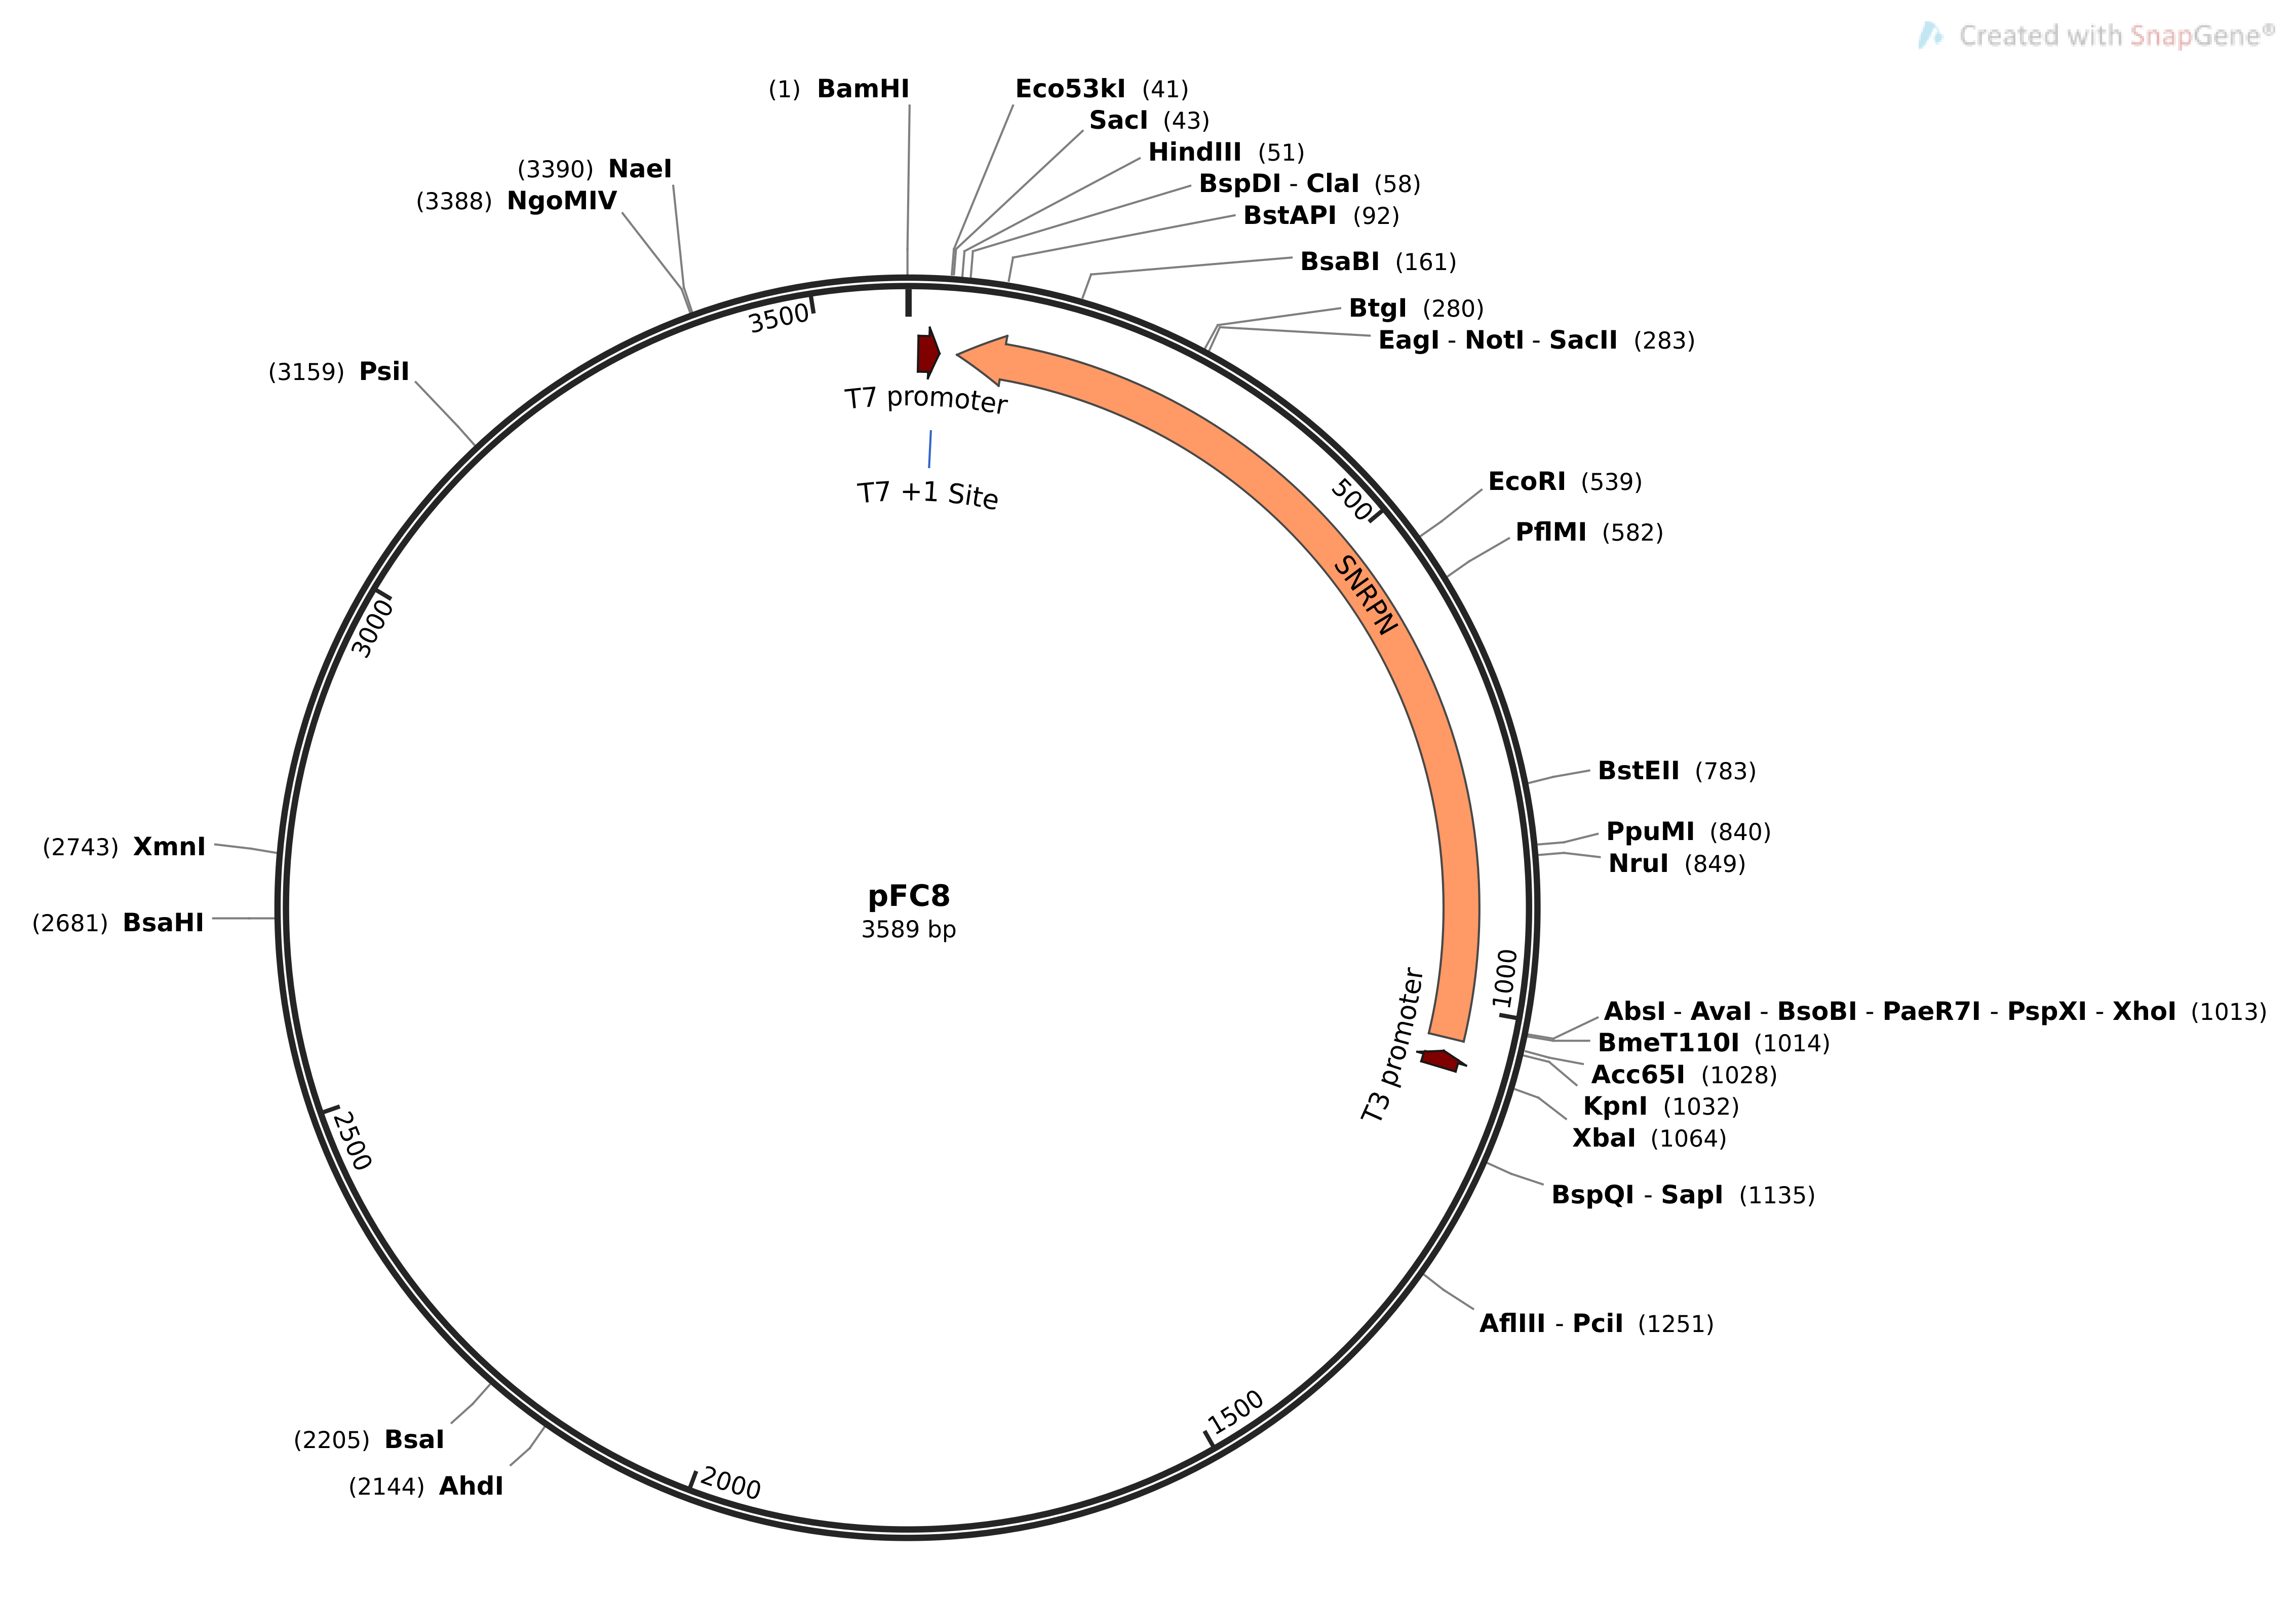
\includegraphics[width=12cm]{images/pFC8_Map.png}
	\centering
	\caption{Map of pFC8.}
	\label{fig:pFC8}
\end{figure}


\begin{figure}[H]
	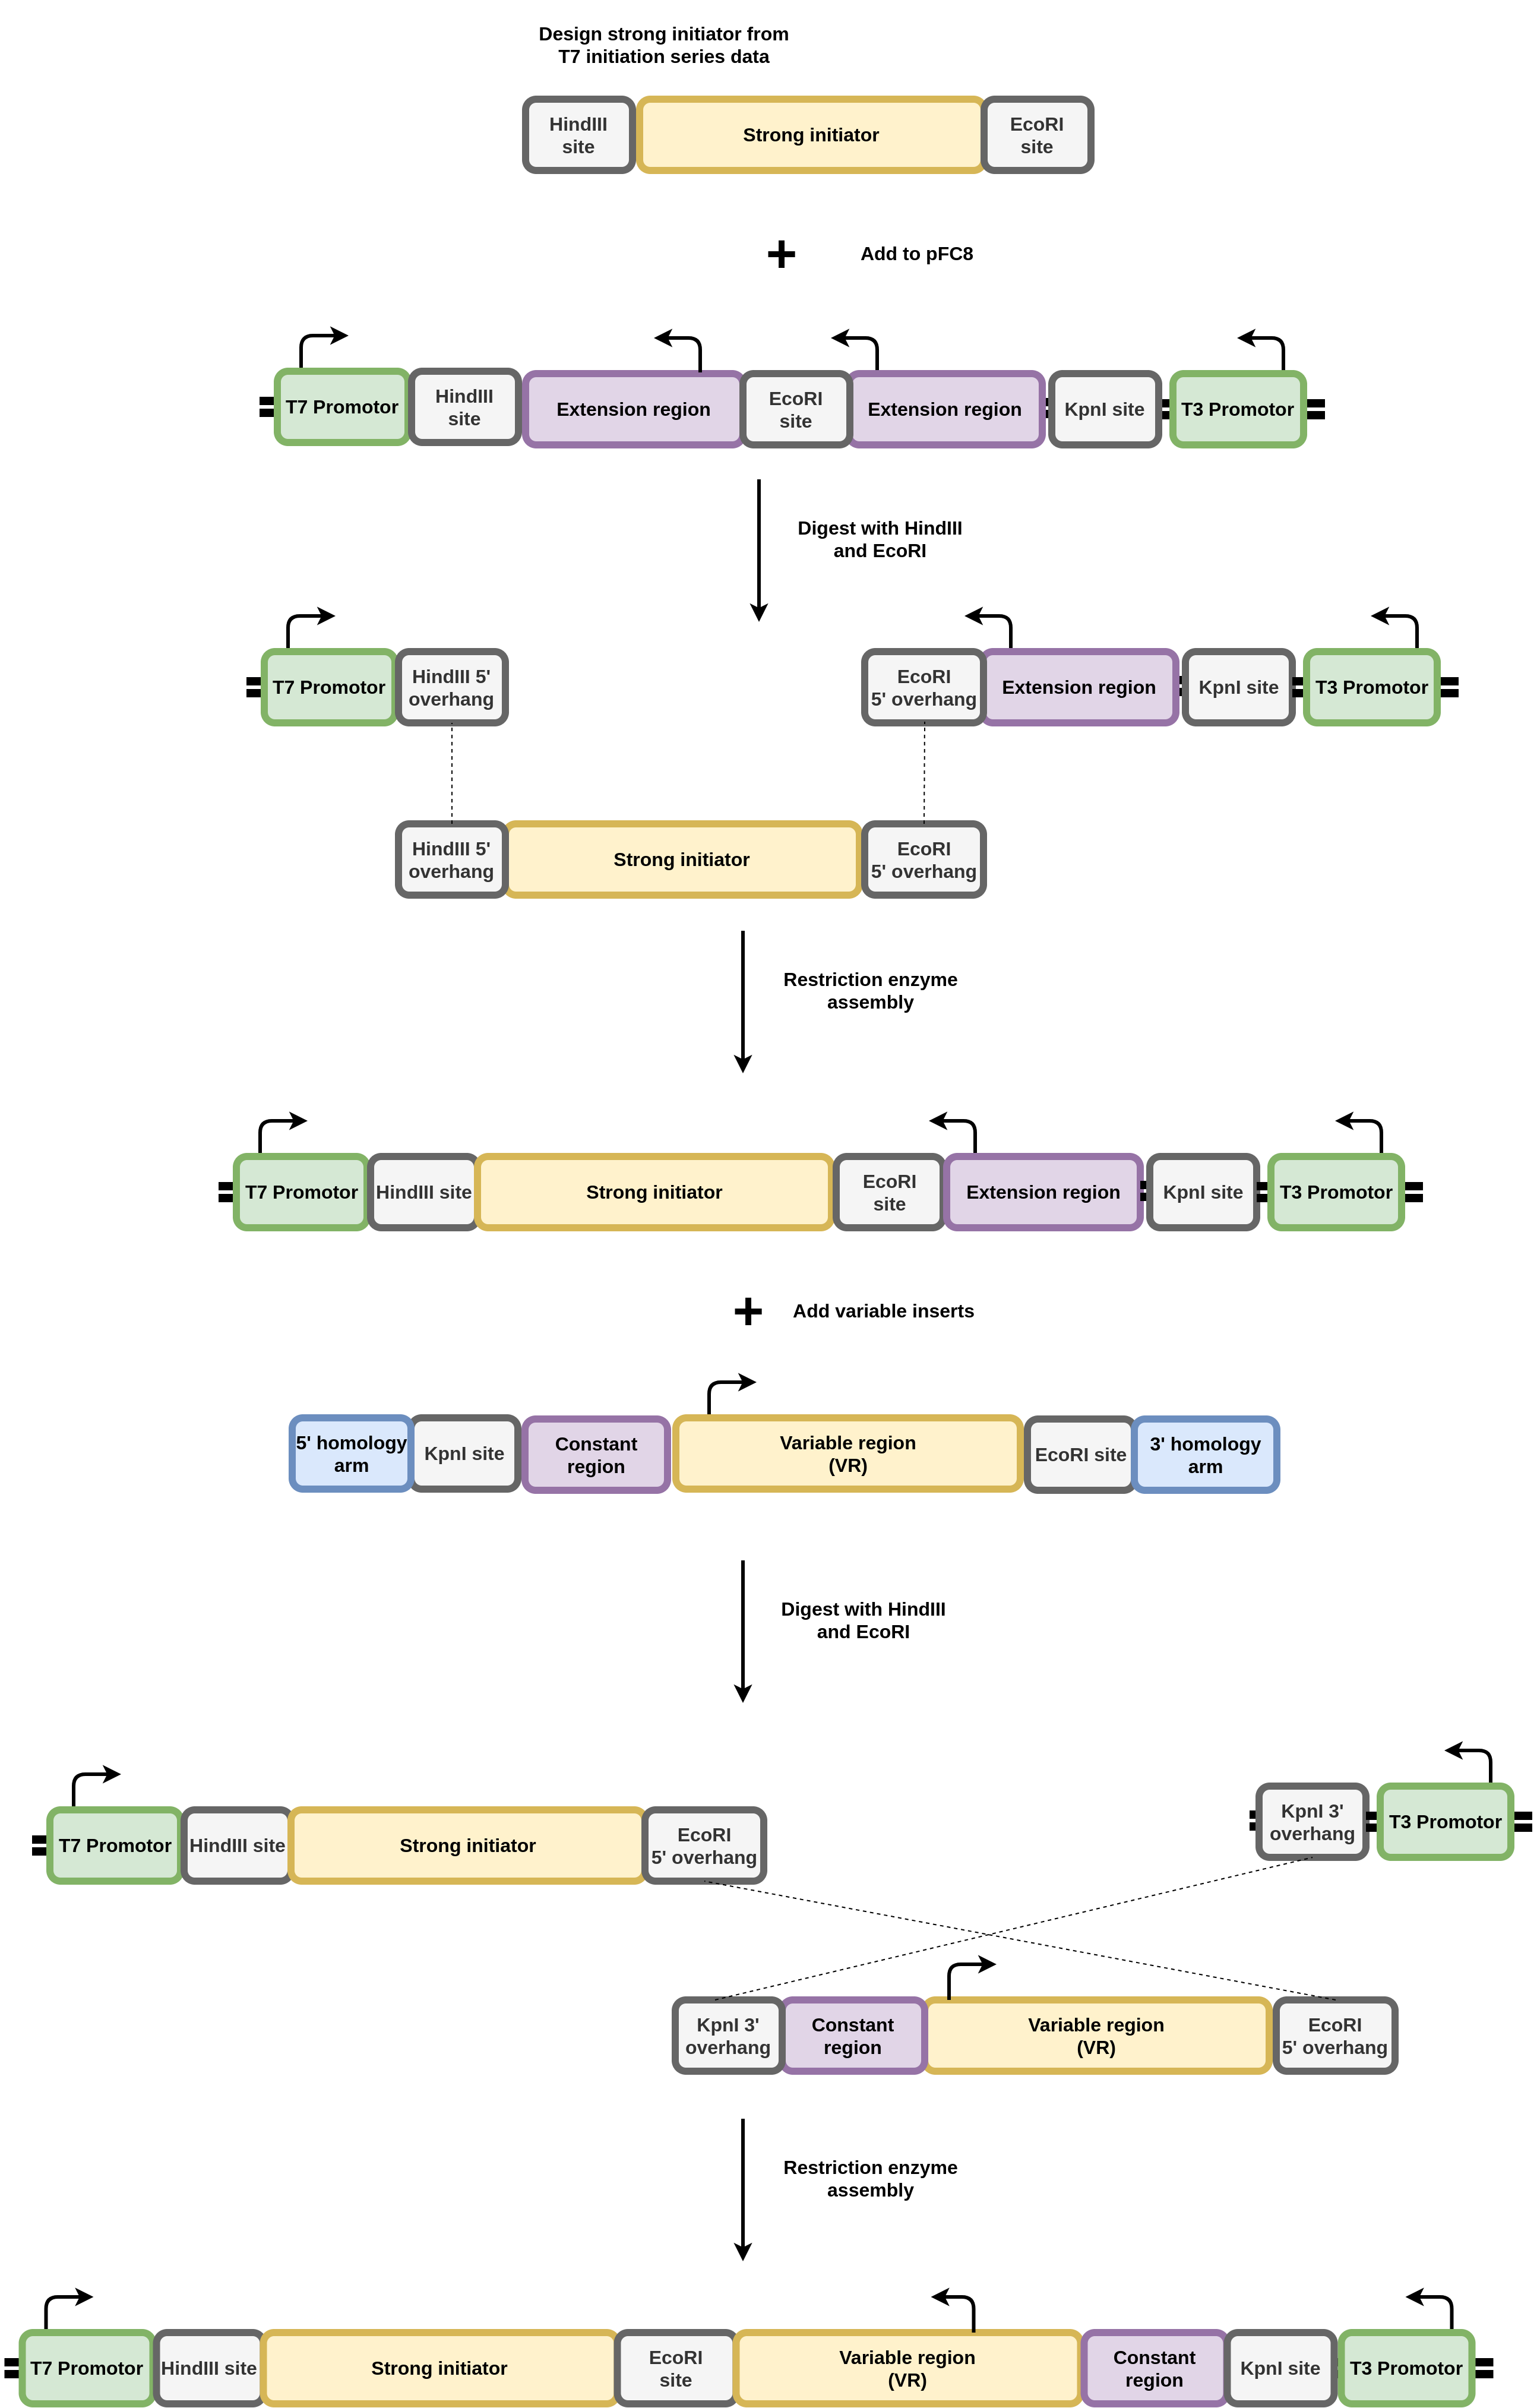
\includegraphics[width=15cm]{images/termination_assembly_pFC8.png}
	\centering
	\caption{Map of pFC9.}
	\label{fig:pFC8_cloning}
\end{figure}


\subsection{Tac initiation series constructs}

\begin{figure}[H]
	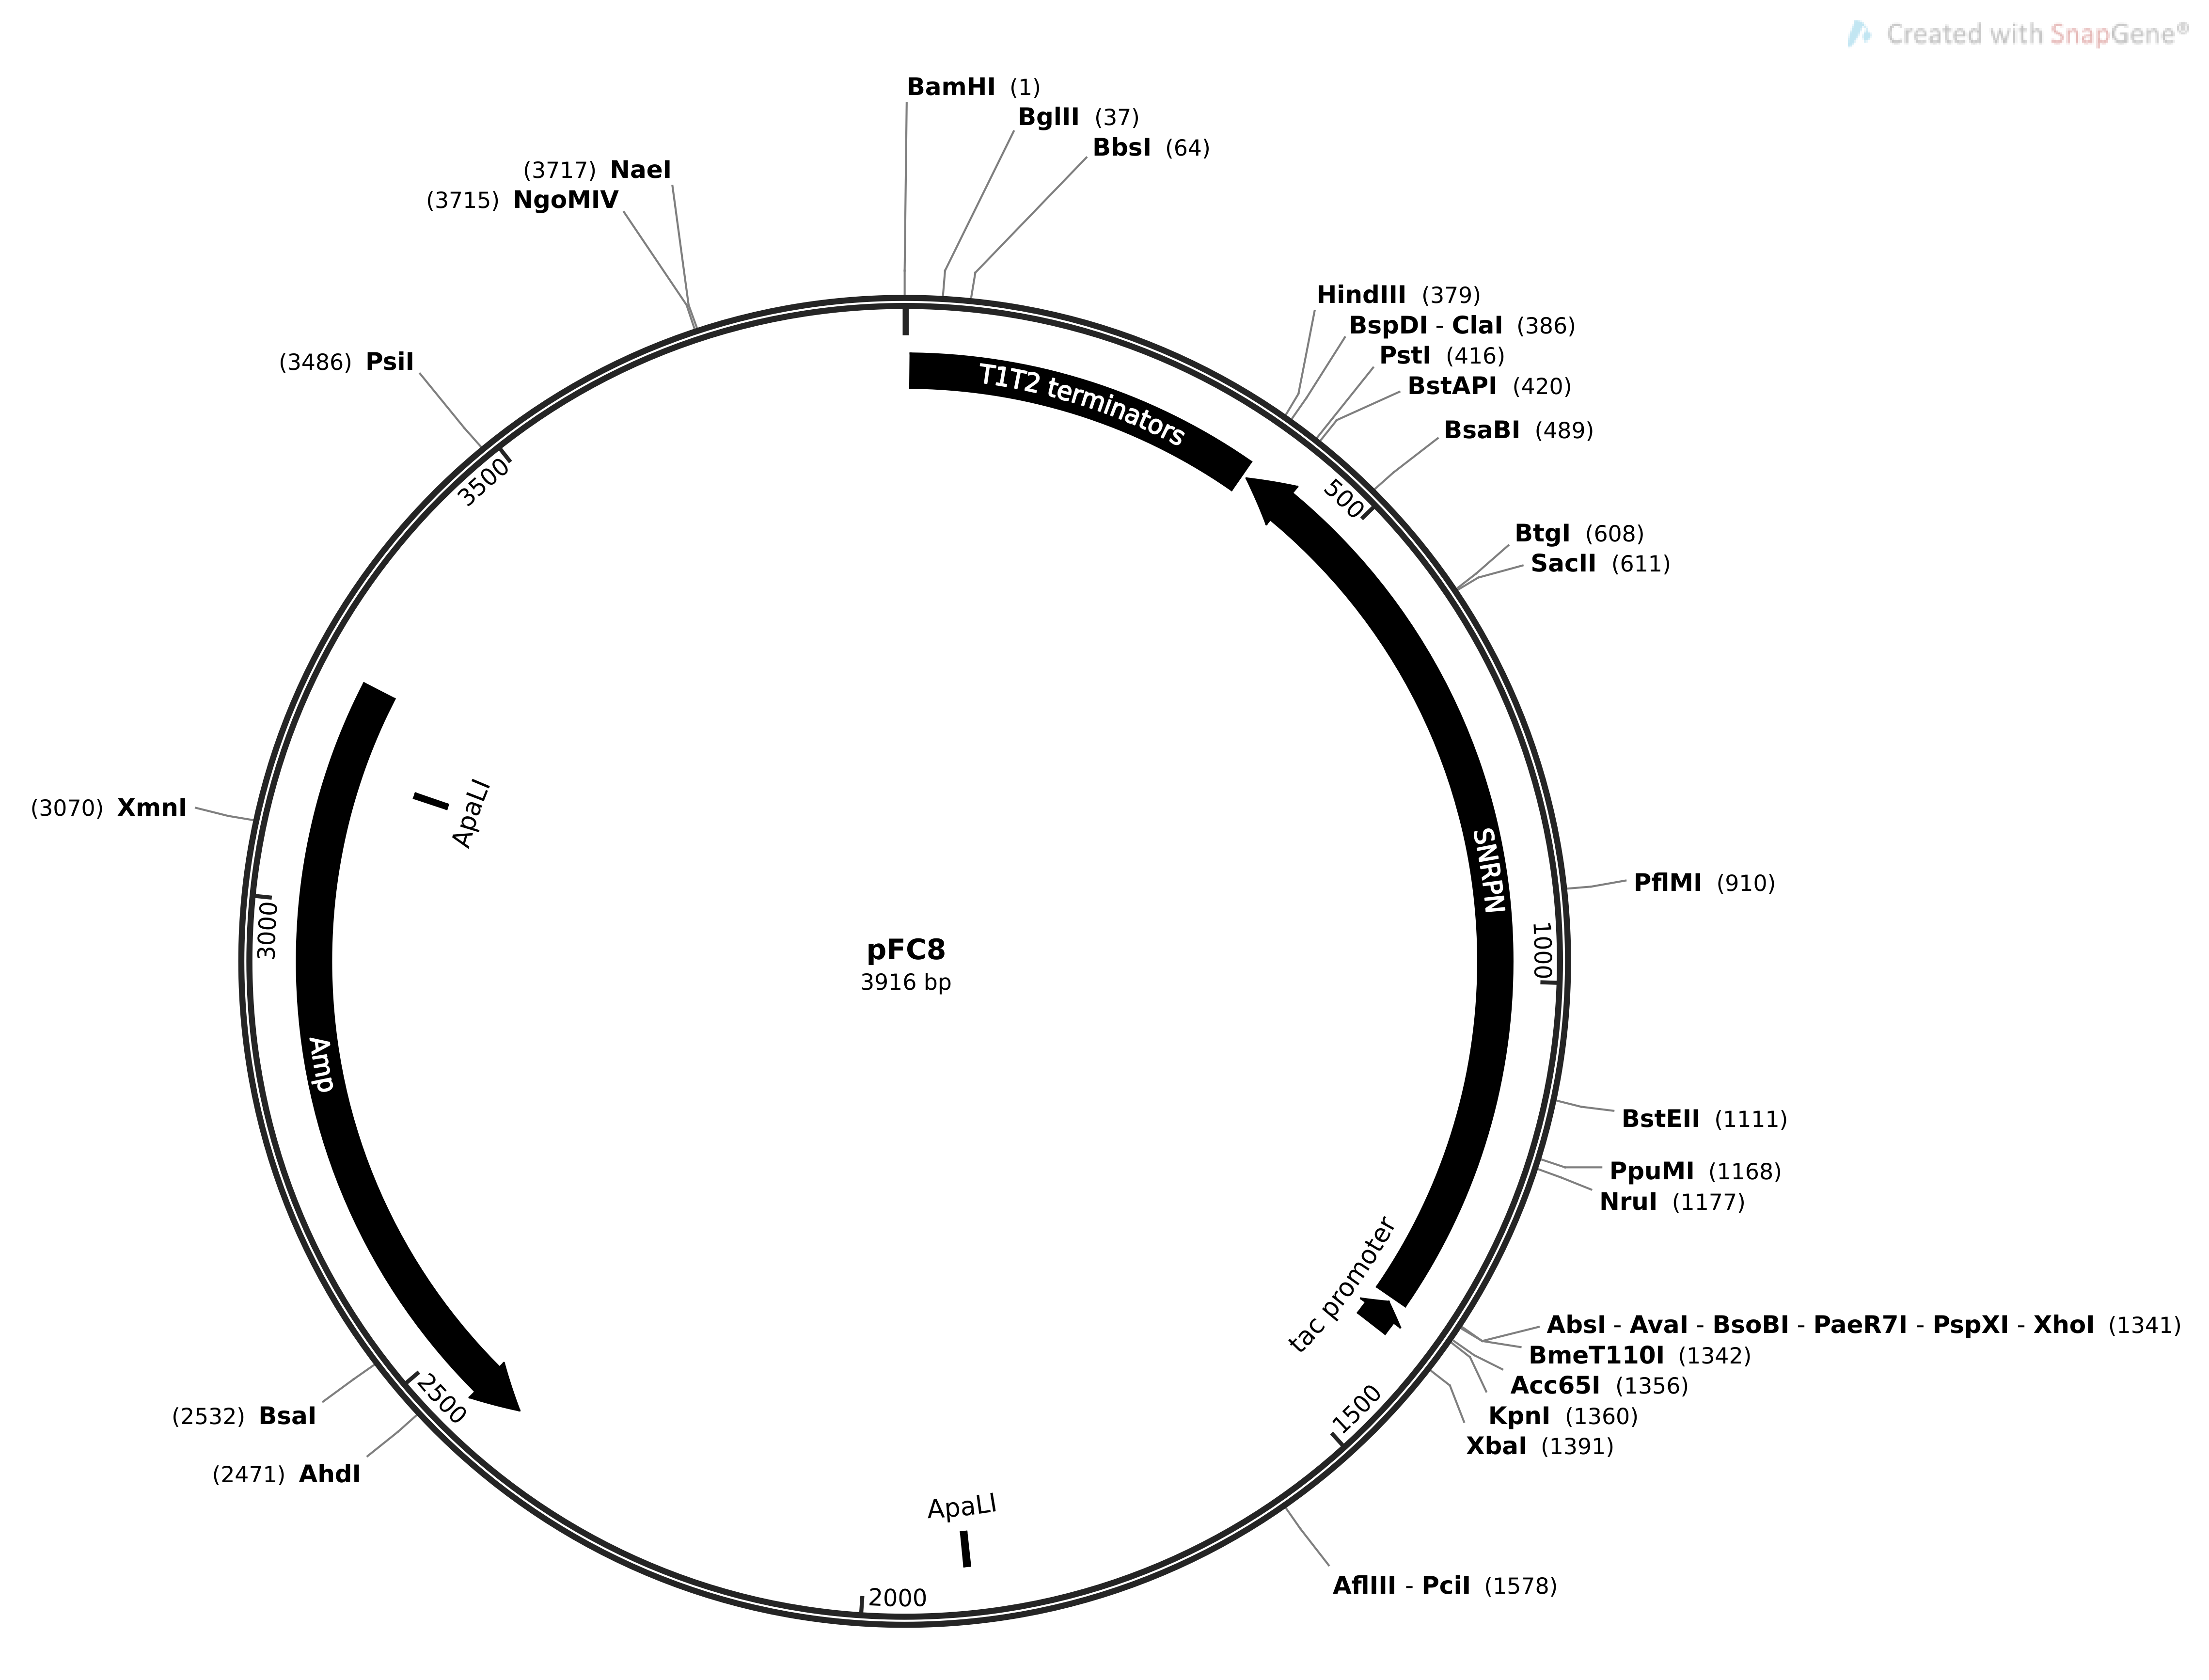
\includegraphics[width=15cm]{images/pFC8tacT1T2_Map.png}
	\centering
	\caption{Map of pFC8T$_1$T$_2$.}
	\label{fig:pFC8T1T2}
\end{figure}

TExt here

\begin{figure}[H]
	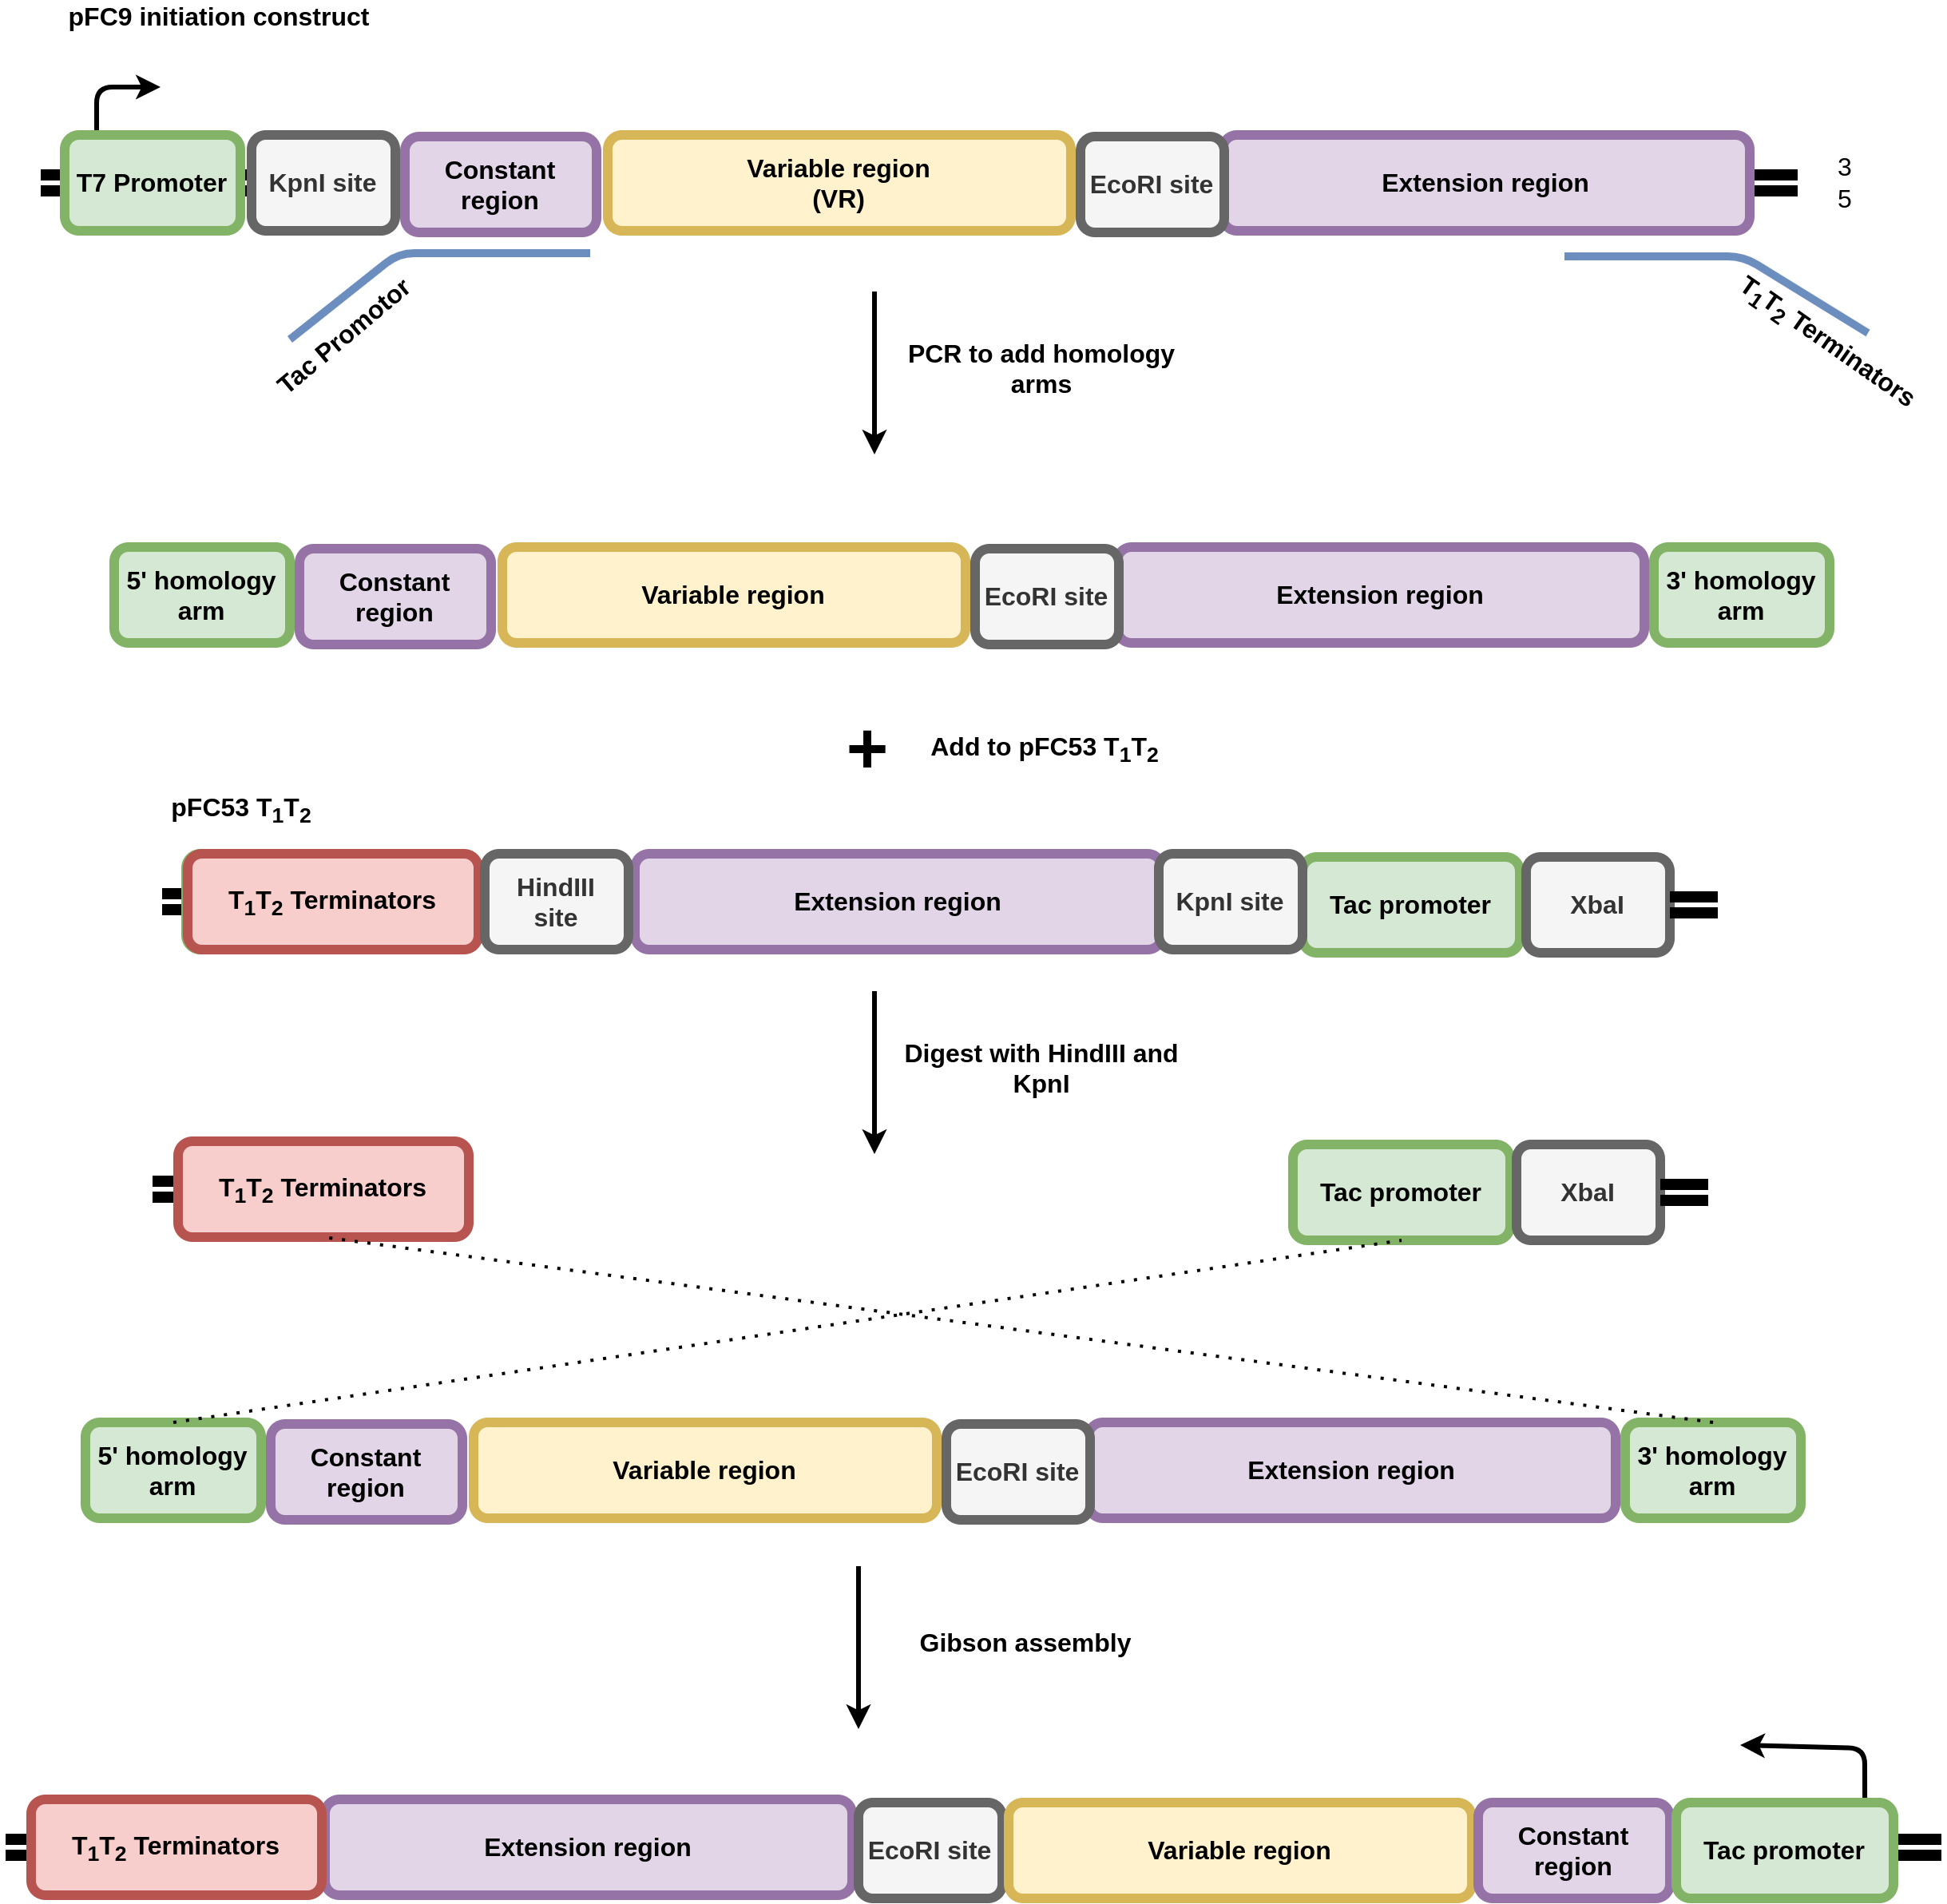
\includegraphics[width=15cm]{images/initiation_assembly_t1t2.png}
	\centering
	\caption{Map of pFC9.}
	\label{fig:pFC8T1T2}
\end{figure}



\subsection{Tac termination series constructs}


\begin{figure}[H]
	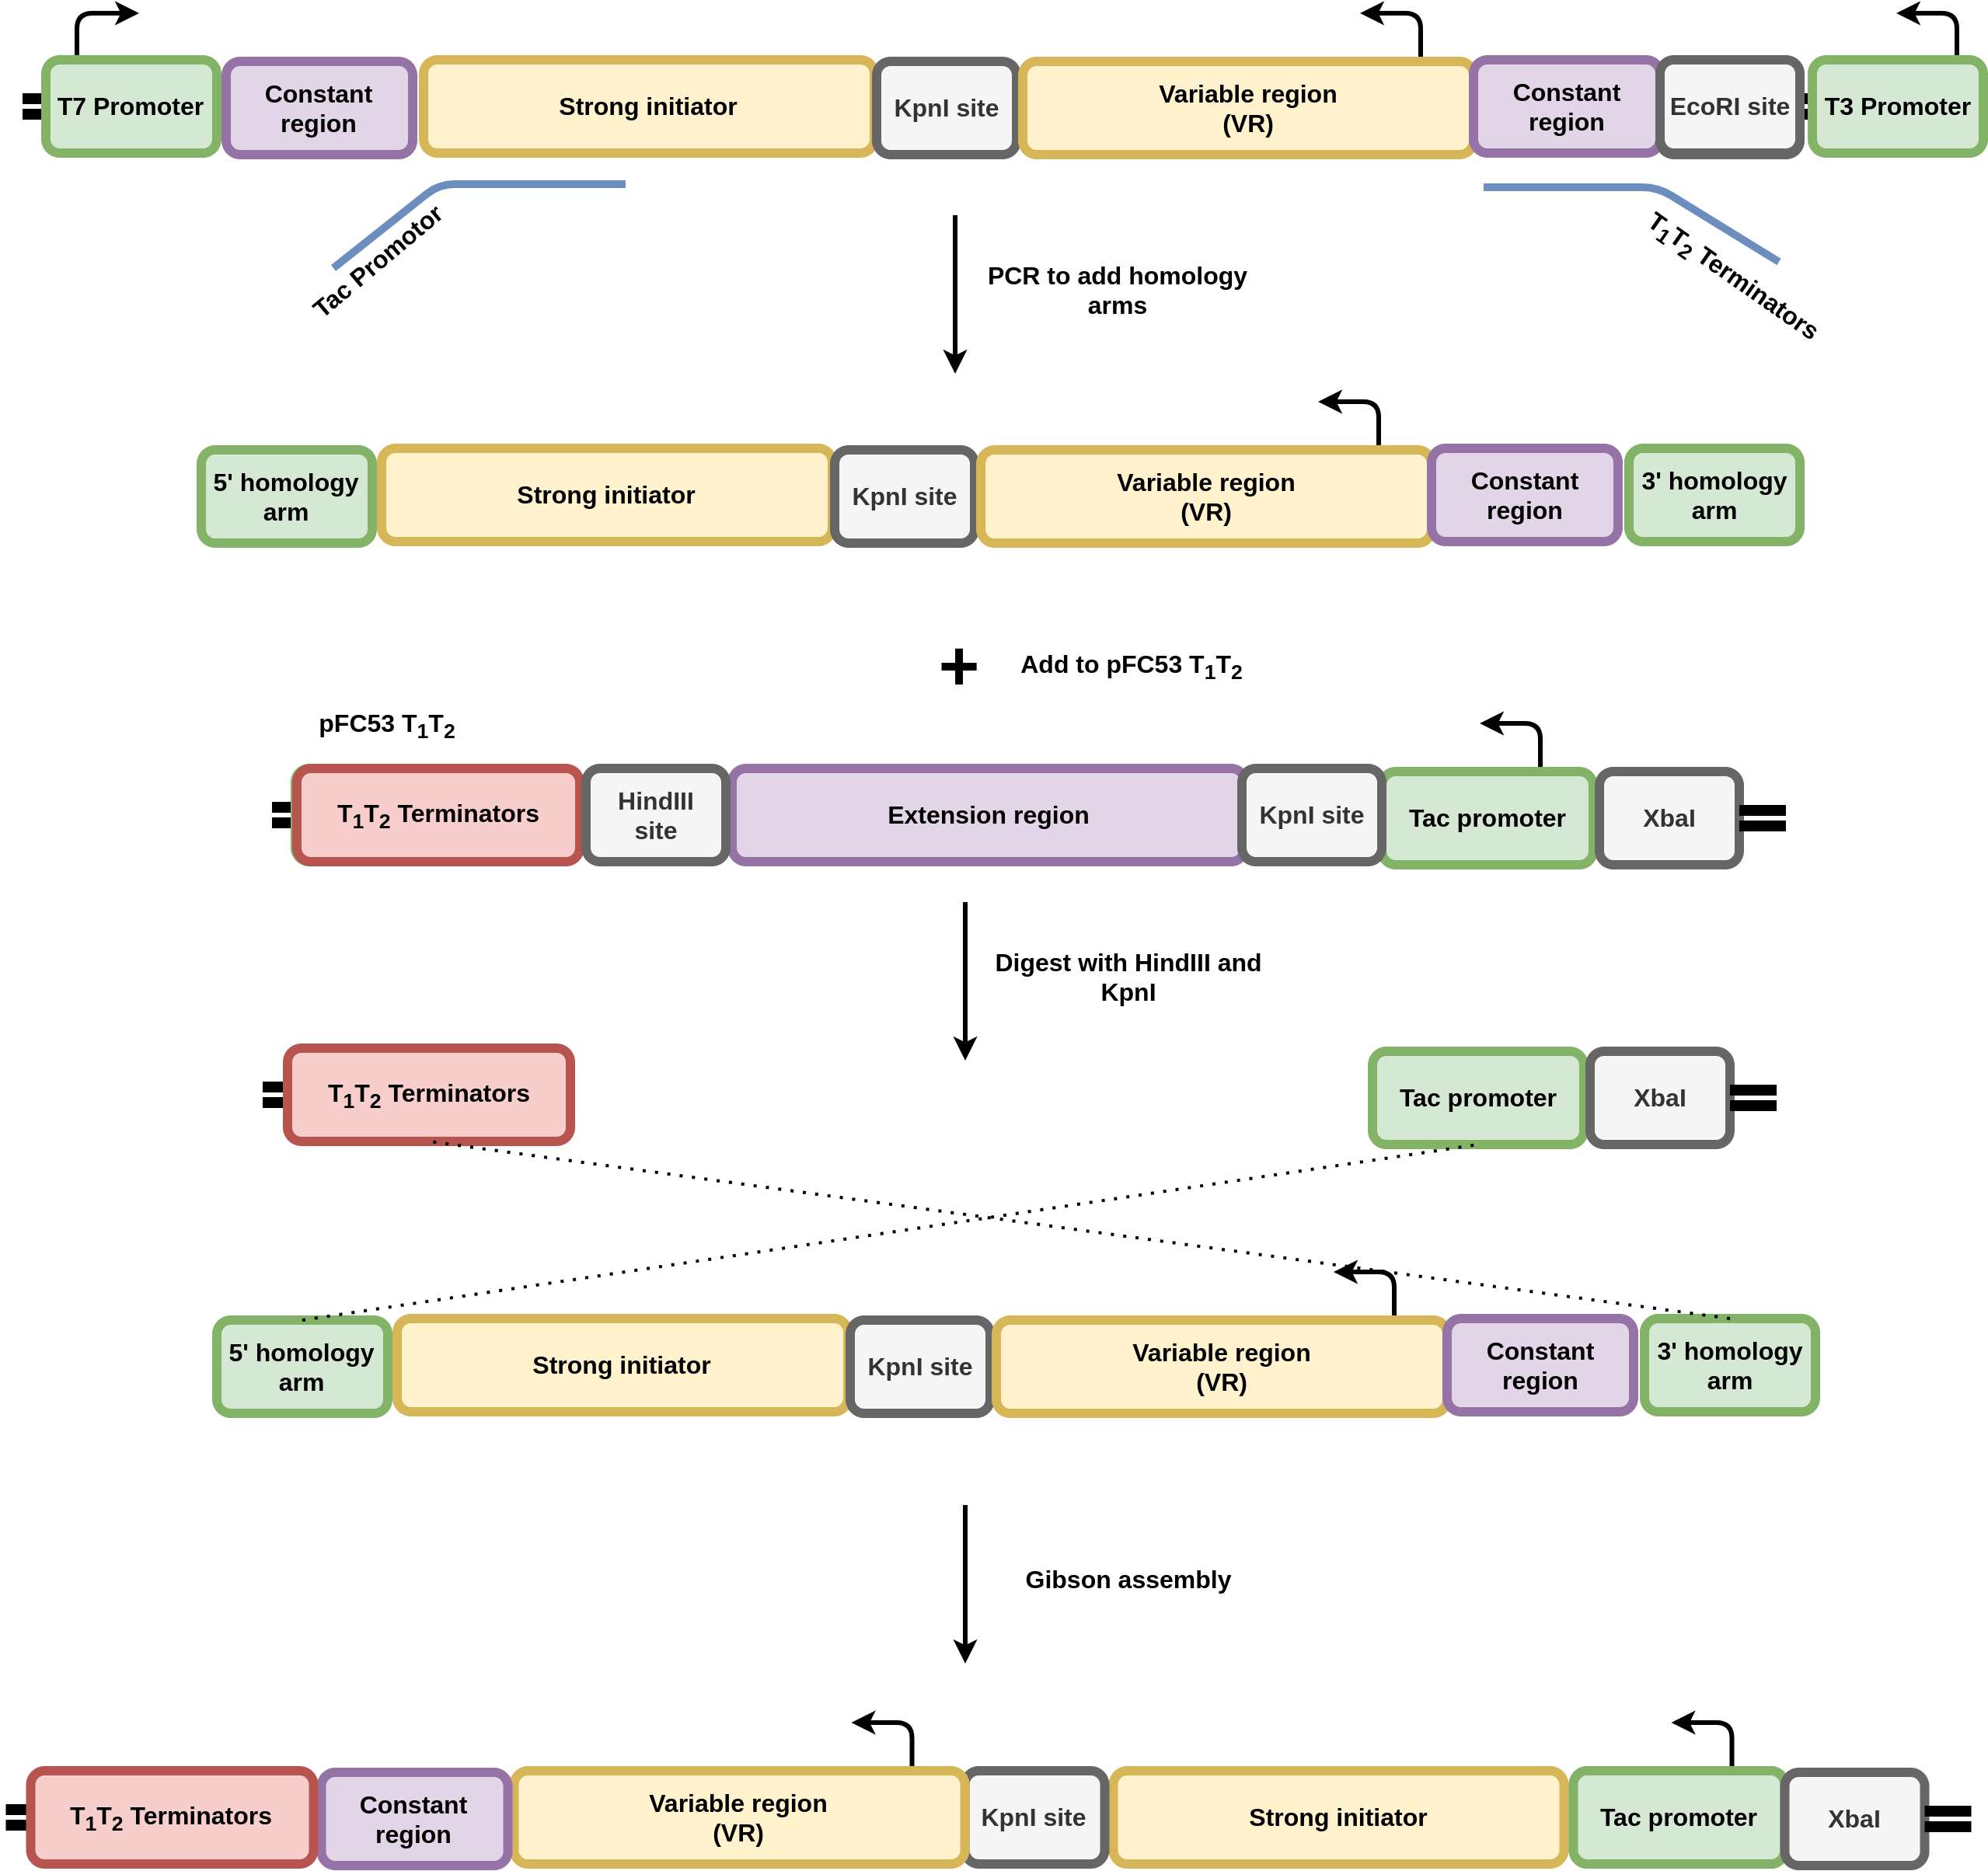
\includegraphics[width=15cm]{images/termination_assembly_pFC53_t1t2.png}
	\centering
	\caption{Map of pFC9.}
	\label{fig:pFC8T1T2}
\end{figure}


\pagebreak

\bibliography{refs/refs.bib}

\end{document}
